\documentclass[12pt]{article}
\usepackage[usenames]{color} %used for font color
\usepackage{amssymb} %maths
\usepackage{amsmath} %maths
\usepackage{graphicx}
\usepackage{url}

\newcommand{\GeV}{\ensuremath{\mathrm{GeV}}}
\newcommand{\TeV}{\ensuremath{\mathrm{TeV}}}
\newcommand{\GeVc}{\ensuremath{\mathrm{GeV}}}
\newcommand{\TeVc}{\ensuremath{\mathrm{TeV}}}
\newcommand{\GeVcc}{\ensuremath{\mathrm{GeV}}}
\newcommand{\TeVcc}{\ensuremath{\mathrm{TeV}}}
\newcommand{\pt}            {\ensuremath{p_{\mathrm{T}}}\xspace}
\newcommand{\kt}            {\ensuremath{k_{\mathrm{T}}}\xspace}
\newcommand{\antikt}        {anti-\kt}
\newcommand{\ttbar}        {\ensuremath{\mathrm{t}\overline{\mathrm{t}}}}
\newcommand{\bbbar}        {\ensuremath{\mathrm{b}\overline{\mathrm{b}}}}
\newcommand{\qqbar}        {\ensuremath{\mathrm{q}\overline{\mathrm{q}}}}
\newcommand{\fbinv}        {\ensuremath{\mathrm{fb}^{-1}}}
\newcommand{\instlumiA}     {\ensuremath{\times 10^{33} \mathrm{cm}^{-2} \mathrm{s}^{-1}}}
\newcommand{\instlumiB}     {\ensuremath{\times 10^{34} \mathrm{cm}^{-2} \mathrm{s}^{-1}}}

\begin{document}

\title{Exascale Computing at the LHC : Narrative}
\author{{\bf Principle Investigators} : \\  
  Reneta Barneva, Matthew Jones, \\ 
  Steven Ko, Salvatore Rappoccio, Lukasz Ziarek \\ \\ 
  {\bf Mentors} : Valentin Brimkov, Peter Elmer}

\maketitle

\clearpage

\section{Funding Strategy}

This research proposal outlines the necessity to extend the computing
capacity of the experiments at the Large Hadron Collider (LHC) in
Geneva, Switzerland, to the exascale of high-throughput
processing. This is an enormously challenging task, but a necessary
one to ensure the long-term success of the LHC experiments. 

Exascale computing (in this case, in high throughput)
is an enormously growth-oriented area. Even during
lean economic times, the US Federal Government is pledging to support
this area of research, for instance in the Department of Energy
Exascale Computing Initiative~\cite{doe_eci}. Indeed, the DOE Office of
Science quotes :
\begin{quote}
The Exascale initiative will be significant and transformative for Department of Energy missions.
\end{quote}
The current level of funding for the DOE EIC and related activities is
\$21M.~\cite{doe_eci_budget}. This ``transformative'' strategy is one
that is envisioned to continue well into the future. 
In addition to DOE programs, the
National Science Foundation (NSF) has several programs to address the
problems of high-throughput exascale computing~\cite{nsf1,nsf2}.

In addition to governmental programs such as above, private sector
funding sources are also available, such as the Google Faculty
Research Awards~\cite{google_fac_awards}, which has an interest in
exascale computing projects also. 

We plan to apply for these projects in the coming year 2013-2014. 


\clearpage

\section{Project Organization}

The principle investigators (PIs) of this proposal have a
widely-varied and applicable skill set to accomplish the goals of
extending LHC computing to the exascale. 

\begin{itemize}
\item Salvatore Rappoccio has 15 years of experience programming in a
high-energy physics environment, as well as other numerical software
design for the private sector. He is an expert in critical
areas of event reconstruction at CMS which can be optimized for
multicore usage. 
\item Lukasz Ziarek has 9 years of experience in language, compiler, and runtime design
targeted at improving multicore performance.  He has worked on 5 compilers and 3 Java VMs. He
is an expert at speculative and transactional computation focusing on the extraction of
parallelism and lightweight concurrency.
\item Steven Ko has 10 years of experience in distributed systems. His recent focus has been large-scale data processing in the cloud using MapReduce and other technologies built on top of it. He also has 5 years of experience in large-scale storage and data management in data centers.
\item Matthew Jones has more than 12 years experience in scientific software development, 
with a particular emphasis on parallel programming.
As the Associate Director of the Center for Computational Research at the University at Buffalo, 
he has also been responsible for designing 
and administering high-performance computing facilites for large-scale
scientific computing.
\item Reneta Barneva has 29 years of experience as a computer
  scientist, and is the author of over 50 publications in the subjects
  of combinatorial image analysis, pattern recognition, and
  computational geometry. 
\end{itemize}

There are also two senior mentors to the project to offer guidance,
insight and technical information. 
\begin{itemize}
\item Valentin Brimkov has over 20 years of experience as a
  mathematician, and has extensive expertise
  in design and analysis of algorithms, combinatorial optimization,
  and discrete geometry. 
\item Peter Elmer is the deputy offline software coordinator of the CMS
experiment at the LHC. He was responsible for the design and implementation
of the data and workflow management system used by CMS, as well as its core
event processing software and software development environment. He has
made important contributions to the software and computing of several 
high-energy physics experiments over the past 20 years and is currently
focused on planning the computing R\&D needed for the next decade in CMS.

\end{itemize}

In addition, the proposal includes funding for
one graduate student from the CSE department at SUNY Buffalo at 100\%
FTE, and one graduate student from the Physics Department at SUNY
Buffalo at 50\% FTE. They will be performing the study of this problem
under the direction of the PIs, and will also be responsible for
deployment and scalability of the solution. 

\clearpage

\section{Narrative}

With the discovery of the Higgs boson 
by the Large Hadron Collider (LHC)
experiments ATLAS and CMS~\cite{higgs_cms,higgs_atlas}, the
standard model (SM) of particle
physics is now complete. This model unifies the electromagnetic force
(carried by the {\em photon}) with the weak force, responsible for
radioactive decay (carried by the {\em $W$ and $Z$ bosons}).
At long last,
physicists now understand that via interactions with the Higgs field,
the $W$ and $Z$ bosons acquire a mass, but the photon does not. 
This is referred to as ``electroweak symmetry breaking''. 


A new phase of particle physics has therefore begun. 
The questions have shifted from the cause of electroweak symmetry
breaking, to the study of the Higgs boson and its interactions in
detail. 
To understand the larger picture of the fundamental forces in nature,
the past excellence of the LHC experiments must therefore continue
unabated in the face of new technical challenges. 


One of the major technical challenges that lies ahead is the
continuation of the scaling of computational power year by year, known
colloquially as ``Moore's Law''. 
To set the scale, at the CMS experiment
with the LHC collision flux (``luminosity'') reaching
$7\instlumiA$, the processing
time to reconstruct each collision event by CMS was approximately 20
seconds per event. However, as the luminosity is
increased, the computational time currently scales quadratically. As
the upgraded LHC is expected to deliver $>12\instlumiA$ in the
upcoming run, the processing time per event is expected to reach
several minutes per event as shown in
Figure~\ref{lumitpeSingleMu}. Furthermore, in future runs of the LHC
in the next 15 years, the luminosity is expected to reach as high as
$>1\instlumiB$, which would correspond (naively) to several hours of
computational time per event! Clearly, it is necessary for the
computing power to scale in order to compensate for this dramatic
increase in CPU time with increasing luminosity. 



However, with the expected end of the historic scaling of single-core
processing capability~\cite{GAMEOVER}, it is imperative to utilize a
parallel processing
strategy in order to maintain the levels of computational speed that
are required.

As a starting point, we first note that during 
2012, the CPU usage for CMS was very 
roughly divided up as:

\begin{itemize}
\item $\sim$40\% event simulation
\item $\sim$20\% prompt event reconstruction (within 48 hours of data-taking)
\item $\sim$40\% mixed user analysis applications
\end{itemize}

Oftentimes,
the codes used by CMS (and experimental HEP in general) tend to lack
clear numerical ``kernels'' where optimization efforts can be focused. 
Given these characteristics they are generally more properly classified as
``high throughput computing'' (HTC) rather than ``high performance computing'' (HPC). 
In terms of their detailed behavior on the CPU many of these codes resemble
more general enterprise or ``cloud''
applications~\cite{CLOUDSUITE,GOODACHEP}.

However, there are several numerical algorithms where parallelization
could be exploited more directly. One of these is the so-called ``jet
clustering'' algorithms used at CMS. 
At CMS, this computation is done very often by individuals rather than
centrally, and so is accounted for
in the 40\% of CPU usage from ``mixed user analysis applications'' as
described above. It is likely, therefore, that improvements observed
in jet clustering will primarily benefit this portion of the CPU
usage. We now discuss the prospects for
utilizing parallelization in jet clustering in detail. 

 

\subsection{Jet Clustering} 




The energetic deposits of particles in detectors need to be clustered
to obtain the
complete response. This is because the process
inherently involves a shower of particles called a ``jet''. This
``jet clustering'' is a well-established technique employed at
many different particle physics experiments worldwide, and is
implemented in a common software framework called 
{\tt fastjet}~\cite{fastjet_manual}. 
The mathematical problem is analogous to the
``K-nearest neighbors algorithm''~\cite{knn_ieee} (kNN). 
The single-core optimization of
jet clustering
is outlined in Ref.~\cite{fastjet_timing}. In a single core,
the computational time scales as $O(N^2)$ or  $O(N \ln{N}$, where $N$
is the number of inputs to the algorithm, which scales linearly with
luminosity. 

There is existing work and literature on the topic of the
parallelization of the kNN algorithm, for instance, in
Refs.~\cite{knn_gpu_1, knn_gpu_2, knn_gpu_3}, where improvements
$O(100)$ in CPU performance are observed over standard
algorithms. Since the proposed use case is
very similar to the kNN algorithm, similar improvements to the
processing time by parallelization strategies are expected. 

We now discuss specific strategies that can be developed in order to
apply to this problem. 

\begin{figure}[h!]
    \centering
    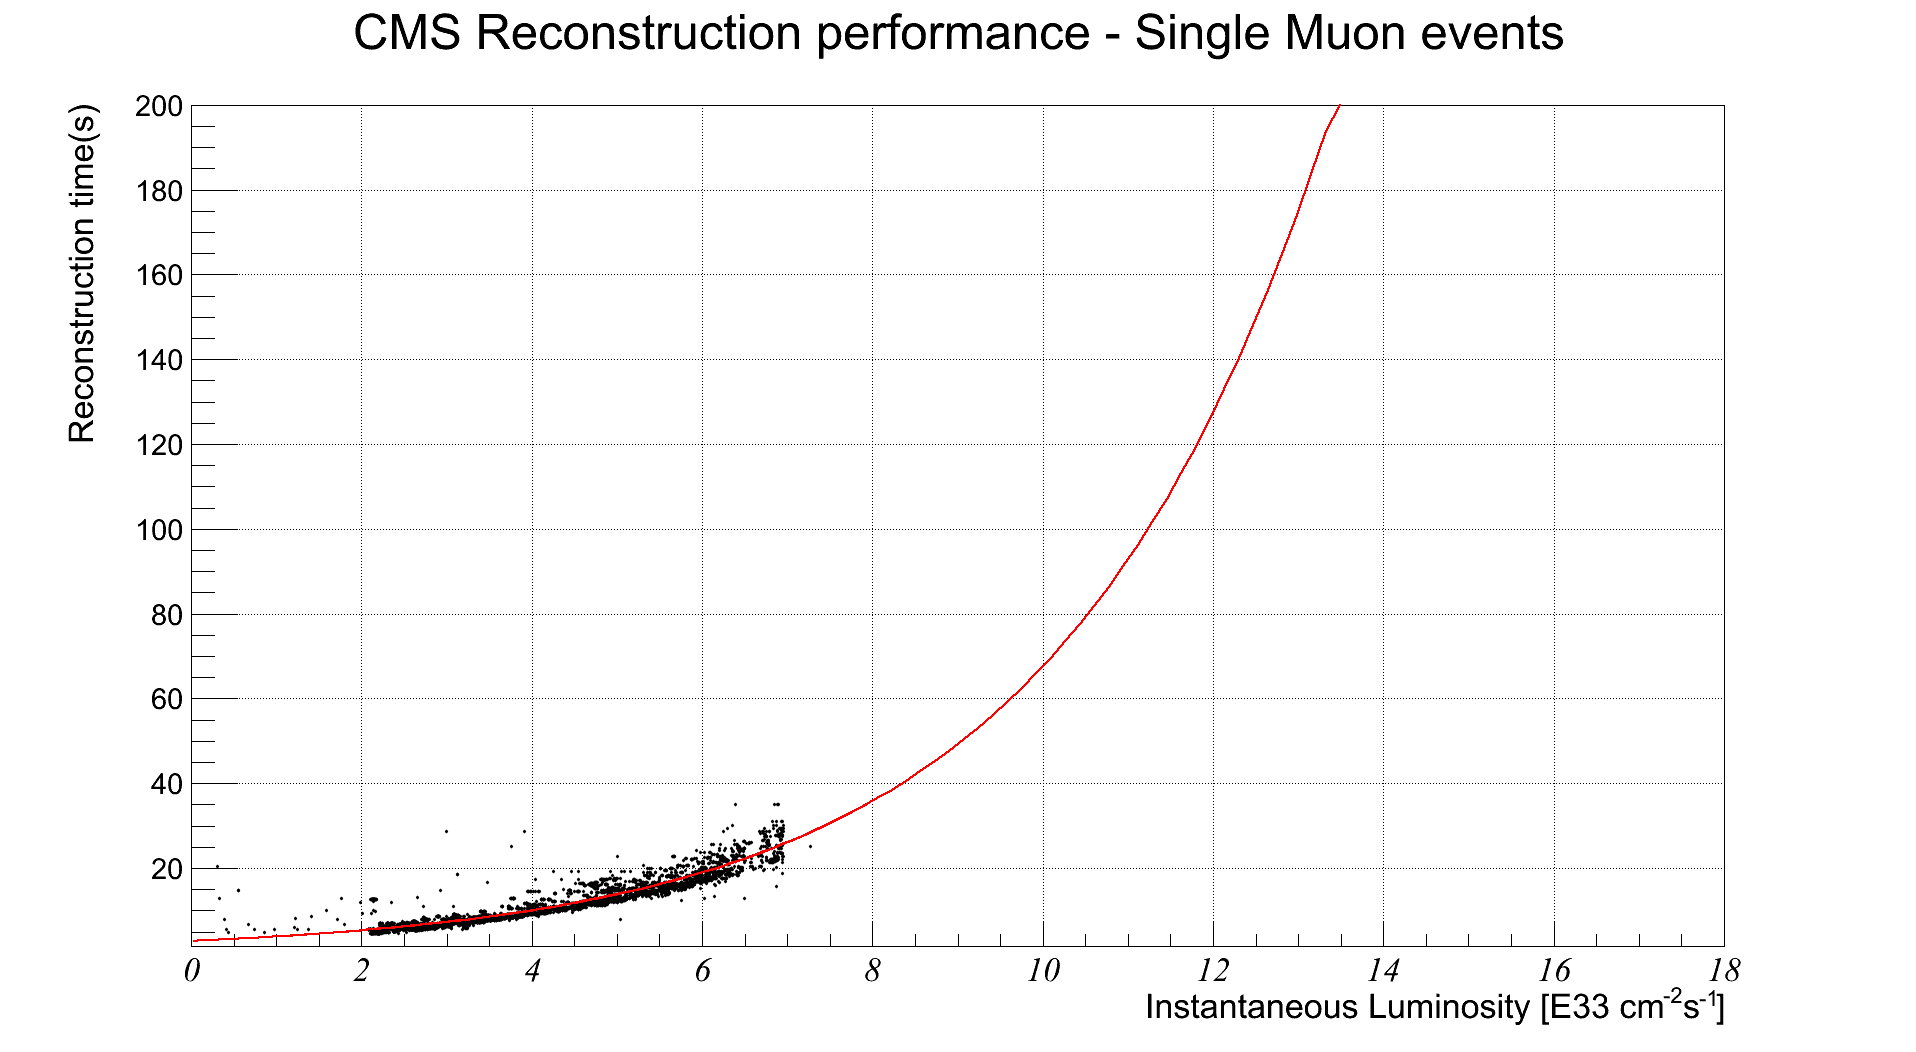
\includegraphics[width=100mm]{lumitpeSingleMu-fitted2.png}
    \caption{\label{lumitpeSingleMu} Event processing time versus
      instantaneous luminosity.}
\end{figure}



\subsection{Full Stack Parallelization}

To achieve the necessary improvements in performance required for scalability
of jet clustering, we propose to examine parallelization opportunities across
the entire software stack, including three specific areas : 
(1) the use of lightweight concurrency
extraction to mask high-latency computations or I/O actions, 
(2) extraction of
parallelization from the computation itself in the form of optimistic speculation
and specialized transform, and
(3) new methods for distributing the computation to
maximize parallelization on each node. 

These three techniques are now discussed in turn. 

\subsubsection{Lightweight Concurrency for Latency Masking}

Many mathematical kernels contain opportunities for extracting ``micro parallelism,''
usually on the order of tens of instructions, from their computational components. 
Unfortunately, it is very difficult to parallelize this computation profitably as
the overhead of thread creation, scheduling, synchronization, and migration outweigh
the gains in parallelism. Instead of extracting explicit parallelism from such
computations, we proposed to explore methods of lightweight asynchrony to allow for
computation to proceed while waiting on high latency I/O operations to complete or
the results of other computations. Since the creation of threads and associated
schedule and synchronization costs are typically prohibitive, we will explore new
threading models that allow for logically-distinct computations to execute within
a given construct. The PIs previous research has indicated that such schemes can profitably
boost overall performance in the context of ML code~\cite{acml, parasites}. The salient research
challenges in applying this strategy are as follows:  1) identifying what computation can be executed
safely during high latency operations at compile time, 2) providing a lightweight threading runtime
and programming model in the context of an imperative language, 
3) specializing the approach to numeric kernels,
and 4) building support for computation in a distributed setting.

\subsubsection{Speculative Computation}

In addition to exploring explicit parallelization of the numeric kernels in jet clustering, we
propose to explore extraction of parallelism via speculative computation. At is core, speculative
computation breaks apart sequential or parallel tasks into smaller tasks to be run in parallel. Once
the speculation has completed, the runtime system validates the computation. If the computation is
incorrect ({\em i.e.} a ``datarace'' is detected, the computation cannot be serialized, {\em etc.}), the
incorrect computation is re-executed in a non-speculative manner.  If the rate of mis-speculation
is low, such techniques can be leveraged to extract additional parallelism. There have been many different
proposals, including large efforts on transactional memory~\cite{}, lock elision~\cite{}, thread level speculation and speculative
multithreading~\cite{},
 for integrating speculative computation into programming languages and their associated runtimes~\cite{}.
The PIs have extensive experience with transactional memory~\cite{trans}, lightweight rollback methods~\cite{stab}, 
leveraging memoization to reduce re-computation costs~\cite{memo1, memo2},
and deterministic speculation~\cite{iso}. We propose to explore a specialized speculation framework leveraging different
speculation strategies, including speculation extracted by the programmer via programming language primitives,
library level speculation, and compiler extracted speculation.
The salient research
challenges in applying this strategy are as follows:  1) identification the appropriate speculation model and
discovering speculation points at compile time, 2) providing a speculative runtime specialized for jet clustering
and capable of realizing user, library, and compiler injected speculation, and 3) exploring new and specialized
lightweight validation and re-execution mechanisms, including validation across multiple speculation strategies.




\subsubsection{Smart Distribution}

\subsection{Summary}

In summary, the problem of expanding LHC computing to the exascale is
a difficult, but tractable one. This proposal investigates the
possibility of applying cutting-edge computer science research to the
real-world application of LHC data processing, specifically by
reducing the computational time for $k$-nearest-neighbor-like
numerical kernels via parallelization. The investigators of this
proposal have extensive experience in the various aspects of the
problem, and the synergistic application of this experience is
expected to attain considerable improvements in this avenue. 

\bibliographystyle{unsrt}
\bibliography{collaborative_proposal}{}
%\bibliography{auto_generated}

\end{document}

% LocalWords:  Exascale LHC Ko Rappoccio Lukasz Zialek Ziarek EIC PIs
% LocalWords:  Collider exascale transformative CMS multicore VMs bla
% LocalWords:  luminosities HEP HTC HPC hadrons hadronic fastjet NN
% LocalWords:  Ref kNN Refs knn gpu factorized workflow MapReduce mis
% LocalWords:  datarace multithreading runtimes memoization
